\section{Оглавление}
(Ссылки кликабельны)\\
\hyperlink{p1}{Задание.....................................................................................................................................................3}\\
\hyperlink{p2}{Выполнение...............................................................................................................................................3}\\
\hyperlink{p4}{Вывод........................................................................................................................................................7}\\
\newpage
\section{Задание}

\hypertarget{p1}1 - Цель работы - на выделенном узле создать и сконфигурировать новый кластер БД Postgres, саму БД, табличные пространства и новую роль, а также произвести наполнение базы в соответствии с заданием. \\
Отчёт по работе должен содержать все команды по настройке, скрипты, а также измененные строки конфигурационных файлов.
Способ подключения к узлу из сети Интернет через helios:
ssh -J sXXXXXX@helios.cs.ifmo.ru:2222 postgresY@pgZZZ
Способ подключения к узлу из сети факультета:
ssh postgresY@pgZZZ
Номер выделенного узла pgZZZ, а также логин и пароль для подключения Вам выдаст преподаватель.

Этап 1. Инициализация кластера БД\\
Директория кластера: \$HOME/qkl81\\
Кодировка: ANSI1251\\
Локаль: английская\\
Параметры инициализации задать через переменные окружения

Этап 2. Конфигурация и запуск сервера БД\\
Способ подключения: сокет TCP/IP, принимать подключения к любому IP-адресу узла\\
Номер порта: 9696\\
Остальные способы подключений запретить.\\
Способ аутентификации клиентов: по паролю MD5\\
Настроить следующие параметры сервера БД:\\
max\_connections\\
shared\_buffers\\
temp\_buffers\\
work\_mem\\
checkpoint\_timeout\\
effective\_cache\_size\\
fsync\\
commit\_delay\\
Параметры должны быть подобраны в соответствии со сценарием OLTP:\\
500 транзакций в секунду размером 4КБ; обеспечить высокую доступность (High Availability) данных.\\
Директория WAL файлов: \$ PGDATA/pg\_wal\\
Формат лог-файлов: .log\\
Уровень сообщений лога: INFO\\
Дополнительно логировать: завершение сессий и продолжительность выполнения команд

Этап 3. Дополнительные табличные пространства и наполнение базы\\
Создать новые табличные пространства для различных таблиц: \$HOME/kdu94, \$HOME/vdk81, \$HOME/ygl69\\
На основе template0 создать новую базу: lazybluelake\\
Создать новую роль, предоставить необходимые права, разрешить подключение к базе.\\
От имени новой роли (не администратора) произвести наполнение ВСЕХ созданных баз тестовыми наборами данных. ВСЕ табличные пространства должны использоваться по назначению.\\
Вывести список всех табличных пространств кластера и содержащиеся в них объекты.\\

Данные, выданные преподавателем: pg116:postgres0:*******
\section{Выполнение}
\hypertarget{p2}
Этап 0:\\
Подключение:\\ ssh -p 2222 s335094@se.ifmo.ru \\ ssh postgres0@pg116\\
\newpage
\textbf{Этап 1:}
Конфигурация
\lstinputlisting[language=SQL]{src/init.sql}
Результат:\\
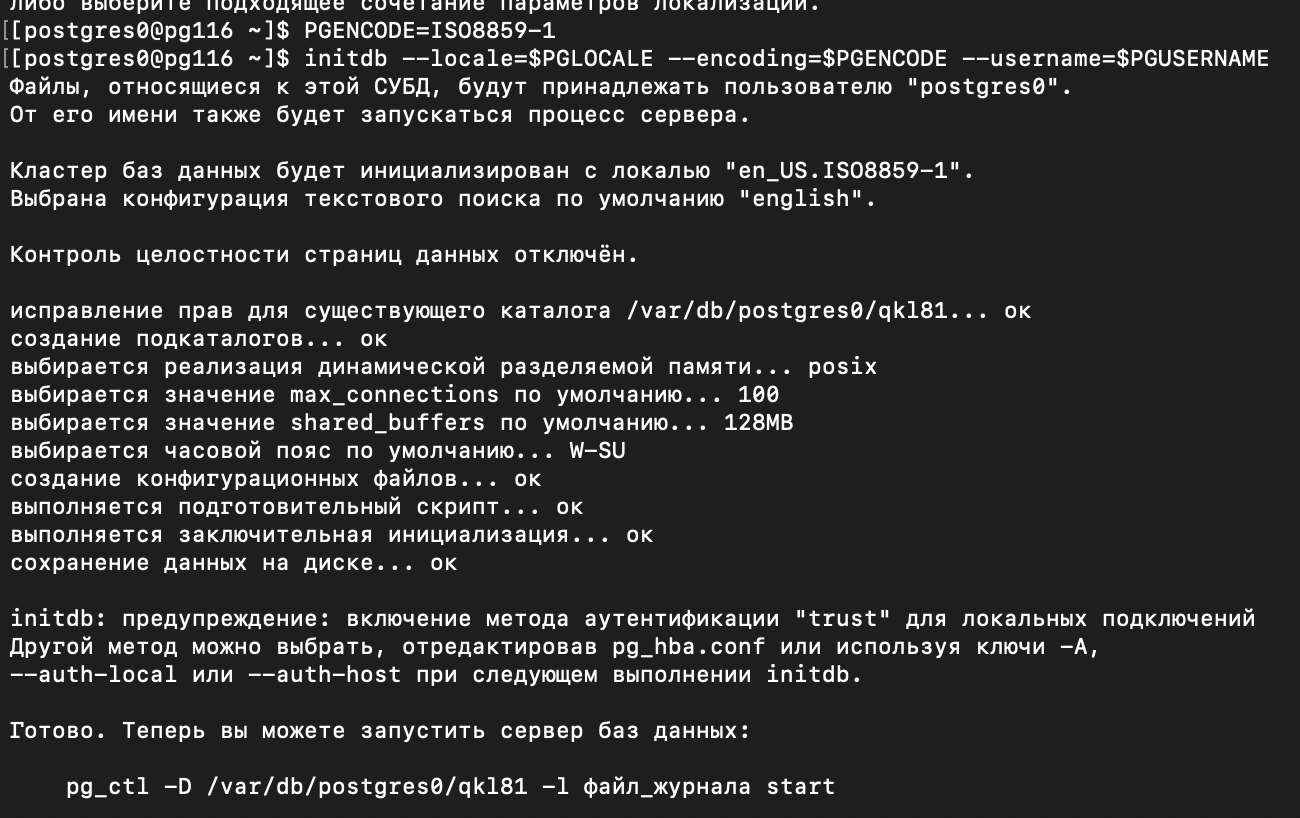
\includegraphics[scale = 0.6]{img/rshd2.png}\\
\textbf{Этап 2:}
Подключение\\
Файл postgresql.conf и его изменения:\\
\lstinputlisting[language=SQL]{src/postgresql.conf}   
Файл pg\_hba.conf и его изменения: \\
\lstinputlisting[language=SQL]{src/pg_hba.conf}   
\textbf{Этап 3:} 
\textbf{Работа с БД \\}
\textbf{Создать новые табличные пространства для различных таблиц: \$HOME/kdu94, \$HOME/vdk81, \$HOME/ygl69\\}

\textbf{На основе template0 создать новую базу: lazybluelake}
\lstinputlisting[language=SQL]{src/lazybluelake_create.bash}
Скрипты для взаимодействия:\\
\lstinputlisting[languagle = SQL]{src/fill.sql}
Вывод:
\lstinputlisting[language=SQL]{src/out.sql}

\section{Вывод}
По итогам выполнения работы я победил создание кластера и его настройку суммарно всего за 13 часов.
\hypertarget{p4}

